\documentclass{article}
\usepackage[utf8]{inputenc}
\usepackage{amsmath}
\usepackage{amsfonts}
\usepackage{graphicx}
\usepackage{listings}

\title{%
    1º Projeto da disciplina Estruturas de Dados II \\
     \large Análise assintótica de algoritmos de ordenação}
\author{Gabriel Passarelli 11218480\\ Marcelo Kenji Noda 11275359\ Danillo Mendes Santiago 10414592}
\date{2021}

\begin{document}
%
\maketitle
%
\newpage
\section{Introdução}
Nosso objetivo com este texto é analisar a complexidade de tempo de cinco algoritmos de ordenação distintos, implementados na parte prática do projeto em linguagem C de programação seguindo os pseudo-códigos fornecidos na proposta do trabalho.\par
%
Em cada seção, fazemos a análise de maneira teórica do pseudo-código de um algoritmo, dando ênfase para o comportamento assintótico da complexidade de tempo, e em seguida apresentamos os resultados obtidos a partir das medições de tempo feitas rodando os códigos implementados. Nessa parte, incluímos gráficos e tabelas para facilitar a visualização dos dados.
%
\section{Análise dos algoritmos}
\subsection{Bubble Sort (versão otimizada)}
O procedimento de ordenação do Bubblesort tem por base comparar elementos adjacentes e invertê-los caso eles estejam desordenados. Percorremos iterativamente o vetor realizando as comparações e as inversões (quando necessárias), e, se percorrermos o vetor sem realizar nenhuma troca, então a rotina termina (e isso distingue o Bubblesort otimizado do normal). Fato é que não caminhamos até o fim do vetor em todo laço, mas sim até uma posição anterior à última que foi atingida no laço anterior, pois, após $i$ rodadas, os $i$ maiores elementos já estarão em suas posições corretas.\par
%
De modo mais preciso, vemos no pseudo-código da rotina Optimized\_Bubble\_Sort que, no pior caso, dado um vetor de tamano $n \in \mathbb{N}$ o número de operações será $n$ vezes o custo do for da linha $4$. Este, por sua vez, realizará aproximadamente 
\[\sum_{i = 0}^{i = n-1}6\cdot(n-i-2) = 3(n - 3)n\] operações em seu interior (a operação de troca normalmente se utiliza de uma variável auxiliar, de modo que o custo dela se torna o custo de 3 atribuições). Ou seja, temos um custo total, no pior caso, $O(n^2)$.\par
O pior caso caso acontece somente quando o vetor está ordenado de maneira decrescente. Tomando um vetor aleatório podemos obter o caso médio. Nessa situação, a probabilidade de que um elemento esteja ocupando uma dada posição no vetor é $1/n$. Perceba que, se esse elemento está deslocado $j$ posições de sua posição correta, então precisaremos realizar pelo menos $j$ trocas para acertá-la. Assim, a questão que precisamos responder então é: em média, quantas posições um elemento está deslocado de sua posição correta? Seja $X_k$, a variável aleatória que mede a distância de um elementos a sua posição correta, quando está é $k$. Temos \[E[X_k] = \sum_{i = 0}^{k-1}\frac{(k-i)}{n}+\sum_{i = k+1}^{n}\frac{(i - k)}{n} = \frac{n+k^{2}+(n-k)^{2}}{2n},\] logo, em um vetor de tamanho $n$, realizaremos \[\sum_{k=0}^{n}E[X_k] = \sum_{k=0}^{n}\frac{n+k^{2}+(n-k)^{2}}{2n} = \frac{(n+1)(n+2)}{3×} = O(n^2)\] permutações.\par
%
Nossas medições de tempo confirmam nossas análises teóricas, como bem se vê pela inclinação das retas do gráfico que compara os quatro algoritmos, inserido no final do relatório.
%
\begin{table}[h]
    \begin{tabular}{c|c|c|c|c|c}
        n = & $10^{1}$ & $10^{2}$ & $10^{3}$ & $10^{4}$ & $10^{5}$ \\ 
        \hline
        Vetor aleatório & $4\cdot 10^{-6}$ & $1.15\cdot 10^{-4}$ & $5.28\cdot 10^{-3}$ & $5.47\cdot 10^{-1}$ & $61.04$ \\
        \hline
        Vetor crescente & $10^{-6}$ & $10^{-6}$ & $5\cdot 10^{-6}$ & $5.1\cdot 10^{-5}$ & $4.61\cdot 10^{-4}$\\
        \hline
        Vetor decrescente & $2\cdot10^{-6}$ & $8.8\cdto10^{-5}$ & $7.3\cdot 10^{-3}$ & $5.3\cdot 10^{-1}$ & $52.12$\\
        \hline
        Média & $2.33\cdot 10^{-6}$ & $6.8\cdot 10^{-5}$ & $4.18\cdot 10^{-3}$ & $3.59\cdot 10^{-1}$ & $37.72$ \\
        \hline
        Desvio Padrão & $1.25\cdot 10^{-6}$ & $4.86\cdot 10^{-5}$ & $3.06\cdot 10^{-3}$ & $2.58\cdot 10^{-1}$ & $26.92$ \\
    \end{tabular}
    \caption{Medidas de tempo para o Bubblesort em segundos}
\end{table}\par
Além disso, observando a tabela, podemos notar como o desvio padrão entre as medições de tempo em cada tipo de entrada cresceu junto com o aumento do tamanho da entrada. Isso reforça nossa avaliação de que a complexidade do BubbleSort está altamente relacionada ao número de elementos já ordenados no vetor inicial.
\subsection{Quick Sort}
Já o Quicksort (C.A.R. Hoare, 1961) usa um método conhecido como "dividir e conquistar" ao escolher um pivô e dividir recursivamente o vetor em dois. Em cada parte do vetor fazemos trocas que garantem que toda chave à esquerda seja menor (para ordem crescente) que o pivô escolhido, seguindo assim para todos subvetores.\par
%
Uma subrotina importante é a que gera partições no vetor $A$, para isso usamos o esquema de Lomuto, um algorítmo tecnicamente mais compacto e fácil de entender, que consiste em escolher o pivô, colocá-lo na ultima posição e percorrer (índice $j$) as chaves anteriores a ele e trocando com $A[i]$ caso $A[j]$ seja menor que o pivô, ao final colocamos o pivô na posição a frente de $i$, então o pivô estará no meio das duas partições. Além deste método, existe também o esquema de Hoare que percorre o subvetor de maneira "cruzada" e algumas variantes que promovem aumento de performance.\par
%
Consideramos que a função partition é a que domina a complexidade, pois as operações de outras subrotinas são despresadas para entradas cada vez maiores no Quicksort. O desempenho deste algorítmo depende fortemente das escolhas de pivô, se elas forem mal balanceadas podemos conseguir o tempo de execução do pior caso $O(n^2)$ pois a rotina de particionamento gera subvetores de $n-1$ e $0$ elementos, então o custo da recursão é \[T(n) = T(n-1) + T(0) + \Omega(n) = \Omega(n) + const + \Omega(n) = \Omega(n^2)\] já para o melhor caso a recusão cria partições de $n/2$ o que, pelo método da árvore de recursões nos dá $T(n) = \Omega(n\cdot log\ n)$. Porém é considerado um excelente ordenador devido a sua eficiência no caso médio $O(n\cdot log n)$ com partições de tamanho aleatório (logo, existe chance de serem bem balanceadas ou não), aplicando o pivô aleatório conseguimos os seguintes tempos de execução: \par

\begin{table}[h]
    \begin{tabular}{c|c|c|c|c|c}
        n = & $10^{1}$ & $10^{2}$ & $10^{3}$ & $10^{4}$ & $10^{5}$ \\ 
        \hline
        Vetor aleatório & $4.0\cdot 10^{-6}$ & $2.8\cdot 10^{-5}$ & $1.9\cdot 10^{-4}$ & $2.2\cdot 10^{-3}$ & $2.8\cdot 10^{-2}$ \\
        \hline
        Vetor crescente & $2.0\cdot 10^{-6}$ & $1.1\cdot 10^{-5}$ & $1.2\cdot 10^{-4}$ & $1.6\cdot 10^{-3}$ & $1.8\cdot 10^{-2}$\\
        \hline
        Vetor decrescente & $2.0\cdot10^{-6}$ & $1.1\cdot 10^{-5}$ & $1.2\cdot 10^{-4}$ & $1.5\cdot 10^{-3}$ & $1.9\cdot 10^{-2}$\\
        \hline
        Média & $2.66\cdot 10^{-6}$ & $1.66\cdot 10^{-5}$ & $1.46\cdot10^{-4}$ & $1.8\cdot 10^{-3}$ & $2.15\cdot 10^{-2}$ \\
        \hline
        Desvio Padrão & $9.42\cdot 10^{-7}$ & $8.01\cdot 10^{-6}$ & $3.25\cdot 10^{-5}$ & $3.2\cdot 10^{-4}$ & $4.4\cdot 10^{-3}$ \\
    \end{tabular}
    \caption{Medidas de tempo para o Quicksort em segundos}
\end{table} \par
%
\subsection{Radix Sort}
A ideia básica por trás do Radixsort é ordenar nossos inteiros de modo recursivo, usando como chave de ordenação uma casa decimal diferente a cada chamada. Comeaçamos pelo dígito menos significativo e terminamos no dígito mais significativo. Cabe dizer que nossas entradas não precisam ser inteiros: datas também funcionariam, ou qualquer outro dado que pudesse ser interpretado como uma sequência de caracteres com uma relação de ordem entre si.\par
%
No pseudo-código, começamos com um vetor $A$ de tamanho $n$. A codição $(maior/posicao)>0$ é a condição de parada do processo de ordenação: $A$ está ordenado quando $posicao$ tiver mais dígitos do que o maior elementos de $A$. Usamos a rotina Counting\_Sort como auxiliar. Ela é responsável por ordenar o vetor $A$ considerando apenas a casa decimal das entradas do vetor de número dado pela fórmula $\log_{10} posicao$. Note que, portanto, o $enquanto$ da linha 4 do peseudo-código rodará um número de vezes igual ao número de dígitos do maior elemento contido em $A$.\par
%
A rotina Counting\_Sort, por sua vez, tem como lógica inferir a posição correta de um dado elemento $a$ de $A$ através da contagem de quantos elementos menores do que $a$ existem em $A$, e é exatamente essa a informação que $B$ guarda: na primeira iteração, contamos quantos elementos de $A$ possuem o dígito especificado pela variável $posicao$ igual a $i$; no segundo laço de iterações contamos também quantos elementos com o dito dígito menor do que $i$ existem em $A$, e salvamos essa informação em $B[i]$. Assim, é evidente que o número correto da posição de $A[i]$ será exatamente $B[chave] - 1$, em que $chave$ é o dígito considerado na chamada atual. Note que a cada iteração, decrementa-se o valor guardado em $B[chave]$, de modo a não se perder os elementos de $A$ com dígito atual igual. No algoritmo, o vetor $C$ serve apenas como auxiliar ao processo de inverção das posições do elemento de $A$.\par
%
Assim, é fácil ver que a complexidade do Radix\_Sort não se altera de acordo com o número de elementos já ordenados no vetor: não fazemos comparações dos elementos entre si, mas sim um procedimento de contagem, cuja complexidade depende apenas do tamanho de $A$. Assim, a complexidade total do algoritmo será, para qualquer vetor de tamanho $n$ \[s\cdot\left[(8 \cdot n + 1) + (1 + 9\cdot4) + (1 + 9\cdot n) + (1 + 3\cdot n)\right] = O(n),\]
em que $s$ corresponde ao número de dígitos do maior elemento do vetor.
%
\begin{table}
    \begin{tabular}{c|c|c|c|c|c}
        n = & $10^{1}$ & $10^{2}$ & $10^{3}$ & $10^{4}$ & $10^{5}$ \\ 
        \hline
        Vetor aleatório & $5\cdot 10^{-6}$ & $3.4\cdot 10^{-5}$ & $2.53\cdot 10^{-4}$ & $3.15\cdot 10^{-3}$ & $3.96\cdot 10^{-2}$ \\
        \hline
        Vetor crescente & $3.0\cdot10^{-6}$ & $1.7\cdot 10^{-5}$ & $2.42\cdot 10^{-4}$ & $3.3\cdot 10^{-3}$ & $3.89\cdot 10^{-2}$\\
        \hline
        Vetor decrescente & $2\cdot10^{-6}$ & $1.8\cdot 10^{-5}$ & $2.43\cdot 10^{-4}$ & $3.12\cdot 10^{-3}$ & $3.89\cdot 10^{-2}$\\
        \hline
        Média & $3.33\cdot 10^{-6}$ & $2.3\cdot 10^{-5}$ & $2.46\cdot10^{-4}$ & $3.2\cdot 10^{-3}$ & $3.92\cdot 10^{-2}$ \\
        \hline
        Desvio Padrão & $1.24\cdot 10^{-6}$ & $7.78\cdot 10^{-5}$ & $4.97\cdot 10^{-6}$ & $7.89\cdot 10^{-5}$ & $3.31\cdot 10^{-4}$ \\
    \end{tabular}
    \caption{Medidas de tempo para o RadixSort em segundos}
\end{table}\par
%
Na tabela, ressaltamos os valores pequenos para o desvio padrão, que indicam que as medidas não se alteraram muito quando mudamos a forma de preencher o vetor a ser ordenado. Isso reforça a ideia de que a complexidade é a mesma para dois vetores quaisquer de mesmo tamanho. Na imagem final, as medições de tempo comprovam o comportamento linear do Radixsort.
\subsection{Heap Sort}
O Heapsort é um algoritmo que se aproveita da estrutura de uma árvore binária para poder otimizar o processo de ordenação. A ideia básica é, dada uma estrutura heap (que no caso é uma árvore cujos nós pais sempre são maiores do que os nós filhos), invertemos, iterativamente, a posição do último nó da árvore com a raiz (que, pelo que dissemos, é o maior nó da árvore). Isso faz com que o último nó passe a ocupar sua posição correta. Contudo, pode ser que essa inversão estrague nossa estrutua de dados, e então a rotina Heapfy é chamada. No próximo laço, invertemos o penúltimo nó, e assim por diante.\par
%
O método Heapfy determina a posição correta de um nó i. Inicialmente, determina-se qual dos nós filhos de i é o maior, e em seguida verifica-se se o valor do nó i é menor do que o do seu maior filho. Se sim, a posição dos dois é trocada, e o método é chamado recursimavente. Se não, siginifica que a rotina terminou. No pior caso, a subárvore do maior nó filho de i conterá $2/3$ do número de nós no total (isso acontece quando a última linha da árvore está preenchida até a metade). Assim, se $T(n)$ é a complexidade do método Heapfy em uma árvore de tamanho n, então \[T(n) = T(2/3n) + c.\]
A solução dessa recursão é $T(n) = c \cdot \log_{2/3}n = O(\ln n).$\par
Evidentemente, apesar de podermos interpretar o vetor $A$, que passamos para o método Heapsort, como uma árvore, ela não necessariamente estará na forma de uma heap, e por isso o procedimento começa com a iteração da linha 2. Essa iteração percorre o penúltimo nível da árvore, fazendo com que cada nó desta seja a raiz de uma heap. Em seguida, vamos para o antepenúltimo nível da árvore, e garantimos novamente que todos os nós desse nível sejam raízes de uma heap, e assim por diante.\par
Na linha 6, inician-se o processo de ordenação da heap, como descrito anteriormente. Pela nossa análise da rotina Heapfy, temos um custo total no pior caso então de \[\left[\frac{n}{2}\cdot(2+O(\ln n)) + 1\right]+ \left[n(3 + O(\ln n) + 3) + 1\right] = O(n\cdot \ln n)\]
Como se vê claramente pelas medições de tempo contidas na tabela, a complexidade de tempo do HeapSort não se altera de maneira relevamente conforme o nível de ordenação prévia da entrada.
%
\begin{table}
    \begin{tabular}{c|c|c|c|c|c}
        n = & $10^{1}$ & $10^{2}$ & $10^{3}$ & $10^{4}$ & $10^{5}$ \\ 
        \hline
            0.000002    0.000016    0.000252    0.003246    0.037669
        Vetor aleatório & $5\cdot 10^{-6}$ & $4.9\cdot 10^{-5}$ & $3.3\cdot 10^{-4}$ & $3.81\cdot 10^{-3}$ & $4.49\cdot 10^{-2}$ \\
        \hline
        Vetor crescente & $2.0\cdot10^{-6}$ & $1.5\cdot 10^{-5}$ & $2.56\cdot 10^{-4}$ & $3.39\cdot 10^{-3}$ & $3.93\cdot 10^{-2}$\\
        \hline
        Vetor decrescente & $2\cdot10^{-6}$ & $1.6\cdot 10^{-5}$ & $2.52\cdot 10^{-4}$ & $3.25\cdot 10^{-3}$ & $3.77\cdot 10^{-2}$\\
        \hline
        Média & $3\cdot 10^{-6}$ & $2.67\cdot 10^{-5}$ & $2.79\cdot10^{-4}$ & $3.48\cdot 10^{-3}$ & $4.19\cdot 10^{-2}$ \\
        \hline
        Desvio Padrão & $1.41\cdot 10^{-6}$ & $1.58\cdot 10^{-5}$ & $3.59\cdot 10^{-5}$ & $2.42\cdot 10^{-4}$ & $4.88\cdot 10^{-3}$ \\
    \end{tabular}
    \caption{Medidas de tempo para o RadixSort em segundos}
\end{table}\par
%
\subsection{Conclusão}
%
\begin{figure}[h]
    \centering
    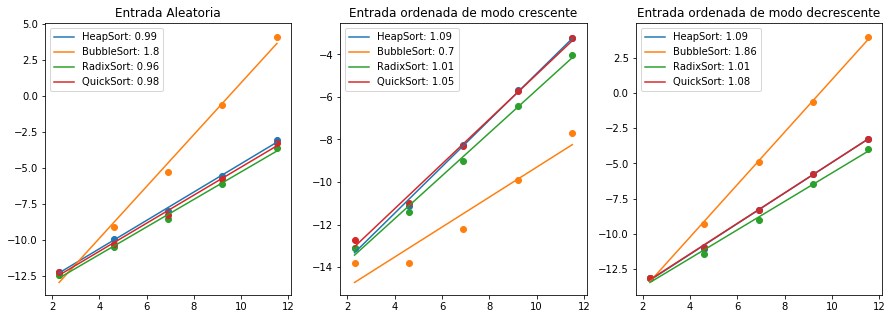
\includegraphics[width=1\textwidth]{comparacao.png}
    \caption{Comparação de tempos entre ordenações (escala logarítmica)}
\end{figure} \par
%
Vemos pelos gráficos que o RadixSort é o algoritmo de ordenação mais eficiente, em média, quando tomamos entradas grandes. Nas análises teóricas, isso se torna evidente, pois, enquanto o Radixsort tem comportamento linear, os demais, excluindo o BubbleSort, têm comportamento $O(n \ln n)$. O BubbleSort tem como ponto positivo sua implementação fácil e rápida; contudo, os gráficos evidenciam que ele se torna inviável para situações em que o mínimo de eficiência no processo de ordenação é requerido. Mais ainda, ele e o QuickSort são ótimos exemplos do porquê se deve realizar a análise de complexidade de tempo de maneira completa: o Bubblesort tem comportamento linear em entradas ordenadas, e o Quicksort, apesar de, nas versões de implementação não randomizada (que não é o caso), ter comportamento quadrático, obteve aqui comportamento de ordem $n\ln n$. Cabe dizer ainda que, apesar de no caso geral, para vetores de qualquer entrada, o RadixSort ter obtido os melhores resultados, devemos notar que sua complexidade de tempo depende da quantidade de caracteres na chave de ordenação, de modo que, então, podem existir situações em que o número de caracteres se torne grande o suficiente para o Radixsort se tornar inferior aos outros métodos. Um exemplo, seria quando se precisa ordenar grandes strings.
%
\end{document}
